% ==============================================================================
%
%                             Dataflow
%
% ==============================================================================
\chapter{Dataflow} \label{chapt:dataflow}
With the Wallis filter implemented on the FPGA the problem becomes that the
image data has to be sent from the computer to the FPGA and back. The following
chapter explains the realiztion of said dataflow. It is split into two main
parts: The communcation and control parts. But before diving into them the
concept of the dataflow is briefly dissected in the following chapter.\\

During the work on the project it was discovered that the initial approach to
the problem would not lead to the optimum solution. This is why a second
implementation was made that differs in both communication and control parts. To
prevent confusion these two solutions are refered to as solution A (the first
approach) and solution B (the second, more performant approach).

% ==============================================================================
%                             Concept
% ==============================================================================
\section{Concept}
As seen in the introduction the image data is sent to the FPGA over Ethernet.
This means on the FPGA side an IP stack has to be implemented to handle Ethernet
communication. The received data then has to be sent to the Wallis filter for
processing and its results to be sent back to the host PC. To distinguish the
data transmission from the dataflow inside the FPGA, the dataflow was split into
two blocks: The communication and control block. The communication block handles
the Ethernet communication while the control block feeds the data in the right
order to the Wallis filter and does houskeeping work. Figure \ref{fig:dataflowa}
shows the dataflow for solution A.
\clearpage
Image data received from the UFT core is stored directly into FPGA block memory
through AXI4 memory mapped interfaces. The UFT core signals a complete file
transfer by asserting \texttt{rx\_done}. This is when the controller starts
reading the data from memory and sending it through AXI4-Stream to the Wallis
filter. The processed data is again stored in block memory. If all data has been
processed, the controller configures the UFT core with the amount of data to
send back and starts the transmission.

\begin{figure}[t!]
    \centering
    \begin{adjustbox}{max width=\textwidth}
        % \tikzsetnextfilename{system-overview}

%-----ABoxes
%-----#1 height, #2 width, #3 aspect, #4 name of the node, #5
%-----coordinate, #6 label
\def\memory[#1,#2,#3,#4,#5]#6{%
  \node[draw, cylinder, alias=cyl, shape border rotate=90, aspect=#3, %
  minimum height=#1, minimum width=#2, outer sep=-0.5\pgflinewidth, %
  color=white!40!black, left color=white!70, right color=white!80, middle
  color=white] (#4) at #5 {};%
  \node at #5 {#6};%
  \fill [white!30] let \p1 = ($(cyl.before top)!0.5!(cyl.after top)$), \p2 =
  (cyl.top), \p3 = (cyl.before top), \n1={veclen(\x3-\x1,\y3-\y1)},
  \n2={veclen(\x2-\x1,\y2-\y1)} in (\p1) ellipse (\n1 and \n2); }

\begin{tikzpicture}[
    rounded corners=0mm,
]
    %coordinates
    \coordinate (ccom)       at (0,0);
    \coordinate (cbram)       at (6,0);
    \coordinate (cip)       at (3,-2);


    %nodes

    \begin{pgfonlayer}{main}

        % Blocks
        \memory[45,40,1.6,bram,(cbram)] {BRAM};

        \node[draw, fill=white, minimum width=3.5cm, minimum height=1cm, anchor=west, text width=2.8cm, align=center] (com) at (ccom) {UFT core};

        \node[draw, fill=white, minimum width=3.5cm, minimum height=1cm, anchor=west, text width=2.8cm, align=center, below = 1cm of bram] (control)  {Controller};

        \node[draw, fill=white, minimum width=3cm, minimum height=1cm, anchor=west, text width=2.8cm, align=center, right = 2cm of control] (ip)  {Image\\Processing};
        
        % Paths
        % UFT to BRAM
        \path[draw,{Latex[length=2.5mm]}-{Latex[length=2.5mm]}] 
            ($(ccom.0) + (3.5,0)$) -- ($(cbram.180) + (-0.7,0.0)$) 
            node [midway, above] () {AXI} ;
        % control to BRAM
        \path[draw,{Latex[length=2.5mm]}-{Latex[length=2.5mm]}] 
            ($(control.0) + (-1.75,0.5)$) -- ($(cbram.180) + (0,-0.7)$) 
            node [midway, right] () {AXI} ;
        % control to ip
        \path[draw,-{Latex[length=2.5mm]}] 
            ($(control.0) + (0,0.3)$) -- ($(ip.180) + (0,0.3)$) 
            node [midway, above] () {Stream} ;
        \path[draw,-{Latex[length=2.5mm]}] 
            ($(ip.180) + (0,-0.3)$) -- ($(control.0) + (0,-0.3)$)
            node [midway, above] () {Stream} ;
        % Control paths
        \path[draw,-{Latex[length=2.5mm]}] 
            ($(control.0) + (-3.5,0)$) -| ($(ccom.0) + (1.75,-0.5)$) 
            node [near start, above] () {control} ;
        \path[draw,-{Latex[length=2.5mm]}] 
            ($(control.0) + (-1.75,-0.5)$) |- ($(control.0) + (0,-1)$) node [near end, above] () {control} -| ($(ip.0) + (-1.75,-0.5)$) 
             ;
        
        % \path[draw,{Latex[length=2.5mm]}-] ($(mon.0) + (0,-0.2)$) -- ($(com.180) + (0,-0.2)$) node[near end, below] () {4.} ;

        % \path[draw,-{Latex[length=2.5mm]}] ($(com.0) + (0,0.2)$) -- ($(ip.180) + (0,0.2)$) node[midway, above] () {2.} ;
        % \path[draw,{Latex[length=2.5mm]}-] ($(com.0) + (0,-0.2)$) -- ($(ip.180) + (0,-0.2)$) node[midway, below] () {3.} ;

    
    \end{pgfonlayer}

    % FPGA box
    \begin{pgfonlayer}{main}
        % \node[above = 0.2cm of com, xshift=-1.5cm] (fpga) { FPGA };
    \end{pgfonlayer}
    \begin{pgfonlayer}{foreground}
        % \node (f_fpga) [draw=black, fill=gray!20, inner sep=20, fit={(com) (ip) }] {};
    \end{pgfonlayer} 

    

\end{tikzpicture}
    \end{adjustbox}
    \caption{Dataflow inside FPGA for solution A}
    \label{fig:dataflowa}
\end{figure}

Following the path of dataflow it is easy to see that the data is stored
multiple
times. In the receiving FiFo of the UFT core, the block memory, then by the
controller in the transmitting and receiving path, again in block memory and in
a Tx FiFo of the UFT transmitter. This cuases latency and high ressource usage.
This is why in a second approach (solution B) the datapath was chosen more
directly. Key element are the AXI4-Stream interfaces. Figure \ref{fig:dataflowb}
shows the new approach using said stream interfaces. The UFT stack outputs
received data comming from the Ethernet line with low latency. The controller
then only buffers the necessary data and starts streaming pixel data to the
Wallis filter as soon as enough data is received. Processed data is buffered in
the controller until the transmitter is ready to send data back.

\begin{figure}[b!]
    \centering
    \begin{adjustbox}{max width=\textwidth}
        % \tikzsetnextfilename{system-overview}

%-----ABoxes
%-----#1 height, #2 width, #3 aspect, #4 name of the node, #5
%-----coordinate, #6 label
\def\memory[#1,#2,#3,#4,#5]#6{%
  \node[draw, cylinder, alias=cyl, shape border rotate=90, aspect=#3, %
  minimum height=#1, minimum width=#2, outer sep=-0.5\pgflinewidth, %
  color=white!40!black, left color=white!70, right color=white!80, middle
  color=white] (#4) at #5 {};%
  \node at #5 {#6};%
  \fill [white!30] let \p1 = ($(cyl.before top)!0.5!(cyl.after top)$), \p2 =
  (cyl.top), \p3 = (cyl.before top), \n1={veclen(\x3-\x1,\y3-\y1)},
  \n2={veclen(\x2-\x1,\y2-\y1)} in (\p1) ellipse (\n1 and \n2); }

\begin{tikzpicture}[
    rounded corners=0mm,
]
    %coordinates
    \coordinate (ccom)       at (0,0);
    \coordinate (cbram)       at (6,0);
    \coordinate (cip)       at (3,-2);


    %nodes

    \begin{pgfonlayer}{main}

        % Blocks
        % \memory[45,40,1.6,bram,(cbram)] {BRAM};

        \node[draw, fill=white, minimum width=3.5cm, minimum height=1cm, anchor=west, text width=2.8cm, align=center] (com) at (ccom) {UFT core};

        \node[draw, fill=white, minimum width=3.5cm, minimum height=1cm, anchor=west, text width=2.8cm, align=center, right = 2cm of com] (control) {Controller};

        \node[draw, fill=white, minimum width=3cm, minimum height=1cm, anchor=west, text width=2.8cm, align=center, right = 2cm of control] (ip)  {Image\\Processing};
        
        % Paths
        % UFT to BRAM
        \path[draw,{Latex[length=2.5mm]}-] 
            ($(ccom.0) + (3.5,-0.3)$) -- ($(control.180) + (0,-0.3)$) 
            node [midway, above] () {Stream} ;
        % control to BRAM
        \path[draw,-{Latex[length=2.5mm]}] 
            ($(ccom.0) + (3.5,0.3)$) -- ($(control.180) + (0,0.3)$) 
            node [midway, above] () {Stream} ;
        % control to ip
        \path[draw,-{Latex[length=2.5mm]}] 
            ($(control.0) + (0,0.3)$) -- ($(ip.180) + (0,0.3)$) 
            node [midway, above] () {Stream} ;
        \path[draw,-{Latex[length=2.5mm]}] 
            ($(ip.180) + (0,-0.3)$) -- ($(control.0) + (0,-0.3)$)
            node [midway, above] () {Stream} ;
        % Control paths
        \path[draw,-{Latex[length=2.5mm]}] 
            ($(control.0) + (-1.45,-0.5)$) |- ($(control.0) + (0,-1)$)  -| ($(ip.0) + (-1.75,-0.5)$)node [near end, right] () {control};
        \path[draw,-{Latex[length=2.5mm]}] 
            ($(control.0) + (-2.05,-0.5)$) |- ($(control.0) + (-3,-1)$) -| ($(ccom.0) + (1.75,-0.5)$) node [near end, left] () {control};
        
        % \path[draw,{Latex[length=2.5mm]}-] ($(mon.0) + (0,-0.2)$) -- ($(com.180) + (0,-0.2)$) node[near end, below] () {4.} ;

        % \path[draw,-{Latex[length=2.5mm]}] ($(com.0) + (0,0.2)$) -- ($(ip.180) + (0,0.2)$) node[midway, above] () {2.} ;
        % \path[draw,{Latex[length=2.5mm]}-] ($(com.0) + (0,-0.2)$) -- ($(ip.180) + (0,-0.2)$) node[midway, below] () {3.} ;

    
    \end{pgfonlayer}

    % FPGA box
    \begin{pgfonlayer}{main}
        % \node[above = 0.2cm of com, xshift=-1.5cm] (fpga) { FPGA };
    \end{pgfonlayer}
    \begin{pgfonlayer}{foreground}
        % \node (f_fpga) [draw=black, fill=gray!20, inner sep=20, fit={(com) (ip) }] {};
    \end{pgfonlayer} 

    

\end{tikzpicture}
    \end{adjustbox}
    \caption{Dataflow inside FPGA for solution B}
    \label{fig:dataflowb}
\end{figure}

% ==============================================================================
%                             Communication
% ==============================================================================
\section{Communication}
The UFT core from project 5 serves as a starting point to the communication
problem. Altough it works on a fundamental basis, the following key features are
missing:

\begin{itemize}
	\item Acknowledgment of received data
	\item Retransmission if a packat was not received
	\item Control interface
	\item Stream based data interface
\end{itemize}

In the following chapters these four problems are addressed and the solutions
explained.

% ==============================================================================
%                             Acknowledge
% ==============================================================================
\subsection{Acknowledge}
The communication is based on the User Datagram Protocol (UDP). This protocol
features low overhead and is simple to implement. The main problem is that the
data sent is not acknowledged hence the sender has no feedback wheather the data
was received or not. This is one reason a custom session protocol (UFT: UDP
File Transfer) was introduced in project 5. It provides command packets for data
packet acknowledgment. Table \ref{tab:uftcommandlist} lists the UFT commands.


\begin{table}[t!]
    \centering
    \begin{tabular}{l l l l l}
        \toprule
        Command & Short & Name & Data 1 & Data 2 \\
        \midrule
        0x00 & FTS & 
        File transfer start & TCID & NSEQ
        \\
        0x01 & FTP &
        File transfer stop & TCID & 0x0000 0000
        \\
        0x02 & ACKFP &
        Acknowledge data packet & TCID & SEQNBR
        \\
        0x03 & ACKFT &
        Acknowledge file transfer & TCID & 0x0000 0000
        \\
        \bottomrule
    \end{tabular}
    \caption{UFT command list}
    \label{tab:uftcommandlist}
\end{table}

The UFT core was extended with the functionality to send acknowledges back to
the PC for data packets and file transfers. For this to work, new connections
inside the UFT block were made. Drawn red in figure \ref{fig:ufttop}, the 
\texttt{uft\_rx\_mem\_ctl} block signals the \texttt{uft\_tx\_ctl} block to send
an acknowledgment. The connection consists of the signals listed in table 
\ref{tab:acksignals}. The tx control block latches the two request signals 
\texttt{ack\_cmd\_nseq} and \texttt{ack\_cmd\_ft} in the case a transmission is
running and an acknowledge request is made. If the tx state machine enters idle
or wait state it checks these latches for an acknowledge request. If a request
is latched, the tx command assembler and tx arbiter are turned on to send an
acknowledge packet. After the packet was sent, the according \texttt{\_done}
signals are asserted.


\begin{figure}[b!]
    \centering
    \begin{adjustbox}{max width=\textwidth}
        % \tikzsetnextfilename{system-overview}
\begin{tikzpicture}[
    rounded corners=0mm,
    entity/.style={
        draw,
        minimum height=1.0cm,
        minimum width=3cm,
        fill=white,
        anchor=north west,
    },
]
    %coordinates
    \coordinate (orig)      at (0,0);
    \coordinate (crx)       at (0,0);
    \coordinate (crxmem)    at (5,0);
    \coordinate (crxamb)    at (10,0);

    \coordinate (ctxctl)    at (0,-2.5);
    \coordinate (ctxcmd)    at (5,-3.5);
    \coordinate (ctxdat)    at (5,-5.5);
    \coordinate (ctxamb)    at (0,-5.5);
    \coordinate (ctxarb)    at (10,-4.5);

    %nodes

    \begin{pgfonlayer}{main}
        % entities
        \node[entity, label={uft\_rx}] (rx) at (crx) {};
        \node[entity, label={[name=rxl] uft\_rx\_mem\_ctl}] (rxmem) at (crxmem) {};

        \node[entity, label={[name=ltxctl] uft\_tx\_ctl}] (txctl) at (ctxctl) {};
        \node[entity, label={[name=txcal]uft\_tx\_cmd\_assembler}] (txcmd) at (ctxcmd) {};
        \node[entity, label={uft\_tx\_data\_assembler}] (txdat) at (ctxdat) {};
        \node[entity, label={uft\_tx\_arbiter}] (txarb) at (ctxarb) {};

        \node[entity, label={axi\_master\_burst}] (ambrx) at (crxamb) {};
        \node[entity, label={axi\_master\_burst}] (ambtx) at (ctxamb) {};

        % ports
        \path[draw,{Latex[length=2.5mm]}-] ($(rx.180) + (0,1/6)$) -- ($(rx.180) + (-1.0,1/6)$) node[anchor=east] {rx\_hdr};
        \path[draw,{Latex[length=2.5mm]}-] ($(rx.180) + (0,-1/6)$) -- ($(rx.180) + (-1.0,-1/6)$) node[anchor=east] {s\_axi};
        \path[draw,{Latex[length=2.5mm]}-] ($(txctl.180) + (0,0)$) -- ($(txctl.180) + (-1.0,0)$) node[anchor=east] {controll};
        \path[draw,{Latex[length=2.5mm]}-] ($(ambtx.180) + (0,0/6)$) -- ($(ambtx.180) + (-1,0/6)$) node[anchor=east] {AXI};

        \path[draw,-{Latex[length=2.5mm]}] ($(ambrx.0) + (0,0)$) -- ($(ambrx.0) + (1.5,0/6)$) node[anchor=west] {AXI};
        \path[draw,-{Latex[length=2.5mm]}] ($(txctl.0) + (0,3.5/10)$) -- ($(txctl.0) + (11.5,3.5/10)$) node[anchor=west] {tx\_hdr};
        \path[draw,-{Latex[length=2.5mm]}] ($(txarb.0) + (0,0/10)$) -- ($(txarb.0) + (1.5,0/10)$) node[anchor=west] {s\_axi};

        % Interconnects
        \path[draw,-{Latex[length=2.5mm]}] ($(rx.0) + (0,1/6)$) -- ($(rxmem.180) + (0,1/6)$) node[anchor=east] {};
        \path[draw,-{Latex[length=2.5mm]}] ($(rx.0) + (0,-1/6)$) -- ($(rxmem.180) + (0,-1/6)$) node[midway, anchor=north] {s\_axi};
        % \node at ($(rx.180) + (-0.5,-1/6)$) [circle,fill,inner sep=1.5pt]{};

        \path[draw,-{Latex[length=2.5mm]}] ($(txctl.0) + (0,1.5/10)$) -| ($(txcmd.180) + (-0.5,0)$) -- ($(txcmd.180) + (0,0)$) node[anchor=west] {};
        \path[draw,-{Latex[length=2.5mm]}] ($(txctl.0) + (0,-1.5/10)$) -| ($(txarb.180) + (-6,0)$) -- ($(txarb.180) + (0,0)$) node[anchor=west] {};
        \path[draw,-{Latex[length=2.5mm]}] ($(txctl.0) + (0,-3.5/10)$) -| ($(txdat.180) + (-1.5,1/6)$) -- ($(txdat.180) + (0,1/6)$) node[anchor=west] {};

        \path[draw,-{Latex[length=2.5mm]}] ($(txcmd.0) + (0,0)$) -| node[anchor=south] {s\_axi} ($(txarb.180) + (-0.5,1/4)$)  -- ($(txarb.180) + (0,1/4)$);
        \path[draw,-{Latex[length=2.5mm]}] ($(txdat.0) + (0,0)$) -| node[anchor=north] {s\_axi}($(txarb.180) + (-0.5,-1/4)$) -- ($(txarb.180) + (0,-1/4)$);

        \path[draw,-{Latex[length=2.5mm]}] ($(ambtx.0) + (0,-1/6)$) -- ($(txdat.180) + (0,-1/6)$) node[anchor=east] {};
        \path[draw,-{Latex[length=2.5mm]}] ($(rxmem.0) + (0,0/6)$) -- ($(ambrx.180) + (0,0)$) node[anchor=east] {};

        % Ack
        \path[draw=red,line width=0.5mm,-{Latex[length=2.5mm]}] ($(crxmem.0) + (1.5,-1)$) |- ($(crxmem.0) + (-1,-2)$) -| ($(ctxctl.0) + (2.5,0)$) node[midway, anchor=east] {};


    \end{pgfonlayer}

    % tx box
    \begin{pgfonlayer}{foreground}
        \node [draw, fill=gray!20, inner sep=10, fit={(ltxctl) (txctl) (txcmd) (txdat) (txarb) (txcal)}, label={[label distance=0.0cm]150:uft\_tx\_top}] (tx) {};
    \end{pgfonlayer} 

    % Board box
    \begin{pgfonlayer}{background}
        \node [draw, fill=gray!40, inner sep=10, fit={(tx) (rx) (rxmem) (rxl)}, label=uft\_top] (tx) {};
    \end{pgfonlayer} 

\end{tikzpicture}
    \end{adjustbox}
    \caption{UFT Top Block Design with acknowledge path}
    \label{fig:ufttop}
\end{figure}


\begin{table}[tb!]
    \centering
    \begin{tabular}{l l l p{8.5cm}}
        \toprule
        Signal & in/out & width & Description \\
        \midrule
        \texttt{ack\_cmd\_nseq} & out & 1 &
        Command to send a data packet acknowledge packet
        \\
        \texttt{ack\_cmd\_ft} & out &1 &
        Command to send a file transfer acknowledge packet
        \\
        \texttt{ack\_cmd\_nseq\_done} & in &1 &
        Asserted if the data packet was acknowledged
        \\
        \texttt{ack\_cmd\_ft\_done} & in &1 &
        Asserted if the file transfer was acknowledged
        \\
        \texttt{ack\_seqnbr} & out & 24 &
        What sequence number to acknowledge
        \\
        \texttt{ack\_tcid} & out & 7 &
        What transaction id to acknowledge
        \\
        \texttt{ack\_dst\_port} & out & 16 &
        Destination port of the host to send the acknowledge to
        \\
        \texttt{ack\_dst\_ip} & out & 32 &
        Destination IP address of the host to send the acknowledge to
        \\
        \bottomrule
    \end{tabular}
    \caption{ACK signals}
    \label{tab:acksignals}
\end{table}

% ==============================================================================
%                             Retransmission
% ==============================================================================
\subsection{Retransmission}
Now that the FPGA sends an acknowledge packet for each data packet, the sending
PC can check if all packets were received by the FPGA. Therefore the PC software
was extended with retransmission. 

Before sending data an array is allocated that will hold the information if a
packet was received. Each element represents a data packet.

\begin{minipage}{\linewidth}
    \begin{lstlisting}[
        style=CStyle, 
        caption=ack buffer allocation, 
        label=lst:ackbufalloc
        ]
    uint8_t *ack_buf = (uint8_t*)malloc( nseq * sizeof(uint8_t) );
    memset(ack_buf, 0, nseq * sizeof(uint8_t));\end{lstlisting}
\end{minipage}

During transmission, the sender checks the receiving buffer for data. If a
acknowledge packet was received, the acknowledge array is updated.

\begin{minipage}{\linewidth}
    \begin{lstlisting}[
        style=CStyle, 
        caption=ack update, 
        label=lst:ackupdate
        ]
    Recv(sockfd, buf, 1500, 0);
    if(get_command(buf) == CONTROLL_ACKFP)
    {
        ack_buf[get_command_ackfp_seqnbr(buf)] = 1;
    }\end{lstlisting}
\end{minipage}

This allows the sending routine to retransmit packets that were not
acknowledged.

% ==============================================================================
%                             Control Interface
% ==============================================================================
\subsection{Control Interface}
The data received by the UFT core in solution A is stored in memory and data to
be sent back
is also located in FPGA memory. To instruct the core to send data, a control
interface is required. Tx base address, data size and rx base address are values
that will be sent from the controller to the UFT core as described later in
chapter \ref{ch:control}. For this purpose a AXI4-Lite slave interface was
realized. AXI4-Lite is a stripped-down version of AXI4. It allows single beat,
memory mapped read and write access from master to slave \cite{axispecs}.

Using Vivados \texttt{Create and Package New IP} command, a 16 register
AXI4-Lite slave interface was generated and connected with the according control
signals of the UFT core. Table \ref{tab:uftaxiregmap} shows the register map.
Registers 8 through 15 can be written by the PC using a custom UFT command
packet. This allows parameters to be sent from PC to FPGA.

\begin{table}[tb!]
    \centering
    \begin{tabular}{l l l p{10cm}}
        \toprule
		Nr & R/W & Offset [hex] & Description \\
        \midrule
		0 & RO & 00 & Status register. Bit 0: \texttt{tx\_ready}. Set if transmitter is
		ready to send data \\
		1 & WO & 04 & Control register. Bit 0: \texttt{tx\_start}. Set 1 to start
		transmitter \\
		2 & WO & 08 & Receiver base address. Received data is stored starting from this
		address \\
		3 & WO & 0C & Transmitter base address. Data to send is read from this address.
		\\
		4 & RO & 10 & Rx counter. Counts how many file transfers were received \\
		5 & WO & 14 & Tx size. How many bytes to send. \\
		6 & & 18 &  Not used\\
		7 & & 1C &  Not used\\
		8 & RO & 20 & User register 0 \\
		9 & RO & 24 & User register 1 \\
		10 & RO & 28 & User register 2 \\
		11 & RO & 2C & User register 3 \\
		12 & RO & 30 & User register 4 \\
		13 & RO & 34 & User register 5 \\
		14 & RO & 38 & User register 6 \\
		15 & RO & 3C & User register 7 \\
        \bottomrule
    \end{tabular}
    \caption{UFT core register map. RO=read only, WO=write only}
    \label{tab:uftaxiregmap}
\end{table}

This new control interface allows the control and status signals from the UFT
core to be read and written using a single normed interface. Figure 
\ref{fig:uftcoreaxilite} shows the complete UFT IP core with AXI4-Lite control
interface, stream and control interface to the UDP core and AXI master burst
interface for memory access (refer to \cite{p5report} for AXI master burst).

\begin{figure}[b!]
    \centering
    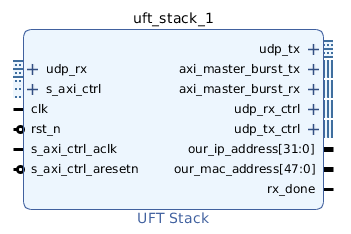
\includegraphics[width=0.5\textwidth] {images/dataflow/uftcoreaxilite.png}
    \caption{UFT core with AXI4-Lite interface}
    \label{fig:uftcoreaxilite}
\end{figure}

% ==============================================================================
%                             Data Interface
% ==============================================================================
\subsection{Data Interface}
The UFT core was in the first place intended for file based data transfer from
PC to FPGA and vice versa. This led to the decision to use memory mapped AXI
interface to store the received data and read the data to be sent. This made
sense with the UFT protocol being file oriented. In the progress of developing
the Wallis filter, a stream based approach was pursued to reduce latency and
memory usage. With the UFT core being memory based, a controller had to be
introduced to send the data from memory to the Wallis filter. Early tests
foreshowed that the UFT core with its memory based interface would be the
limiting member in the data processing chain. So the core's data interface was
rewritten to support AXI4-Stream for data receiving and sending.

For solution B, the two \texttt{axi\_master\_burst} blocks were removed and the
code of the \texttt{uft\_rx\_mem\_ctl} and \texttt{uft\_tx\_data\_assembler}
changed to directly connect the AXI4-Stream from the UDP stack to the outside.
Advantage of this solution is the reduced latency and less memory usage. One
downside is that the receiver is no longer able to reorder packets if they do
not arrive in order. As long as the application runs on a closed network it can
be assumed that packets will not change order.

\begin{figure}[b!]
    \centering
    \begin{adjustbox}{max width=\textwidth}
        % \tikzsetnextfilename{system-overview}
\begin{tikzpicture}[
    rounded corners=0mm,
    entity/.style={
        draw,
        minimum height=1.0cm,
        minimum width=3cm,
        fill=white,
        anchor=north west,
    },
    entityold/.style={
        draw=gray!60,
        minimum height=1.0cm,
        minimum width=3cm,
        fill=gray!20,
        anchor=north west,
    },
]
    %coordinates
    \coordinate (orig)      at (0,0);
    \coordinate (crx)       at (0,0);
    \coordinate (crxmem)    at (5,0);

    \coordinate (ctxctl)    at (0,-2.5);
    \coordinate (ctxcmd)    at (5,-3.5);
    \coordinate (ctxdat)    at (5,-5.5);
    \coordinate (ctxarb)    at (10,-4.5);
    \coordinate (caxilite)  at (-5,-2.5);

    \coordinate (ctxamb)    at (0,-5.5);
    \coordinate (crxamb)    at (10,0);
    %nodes

    \begin{pgfonlayer}{main}
        % entities
        \node[entity, label={uft\_rx}] (rx) at (crx) {};
        \node[entity, label={[name=rxl] uft\_rx\_mem\_ctl}] (rxmem) at (crxmem) {};

        \node[entity, label={[name=ltxctl] uft\_tx\_ctl}] (txctl) at (ctxctl) {};
        \node[entity, label={[name=txcal]uft\_tx\_cmd\_assembler}] (txcmd) at (ctxcmd) {};
        \node[entity, label={uft\_tx\_data\_assembler}] (txdat) at (ctxdat) {};
        \node[entity, label={uft\_tx\_arbiter}] (txarb) at (ctxarb) {};

        \node[entityold, label={axi\_master\_burst}] (ambrx) at (crxamb) {};
        \node[entityold, label={axi\_master\_burst}] (ambtx) at (ctxamb) {};

        % ports
        \path[draw,{Latex[length=2.5mm]}-] ($(rx.180) + (0,1/6)$) -- ($(rx.180) + (-1.0,1/6)$) node[anchor=east] {rx\_hdr};
        \path[draw=blue,line width=0.5mm,{Latex[length=2.5mm]}-] ($(rx.180) + (0,-1/6)$) -- ($(rx.180) + (-1.0,-1/6)$) node[anchor=east] {s\_axi};
        \path[draw,{Latex[length=2.5mm]}-] ($(txctl.180) + (0,0)$) -- ($(txctl.180) + (-1.0,0)$) node[anchor=east] {controll};

        \path[draw=blue,line width=0.5mm,-{Latex[length=2.5mm]}] ($(rxmem.0) + (0,0)$) -- ($(rxmem.0) + (6.5,0/6)$) node[anchor=west] {s\_axi\_rx};
        \path[draw,-{Latex[length=2.5mm]}] ($(txctl.0) + (0,3.5/10)$) -- ($(txctl.0) + (11.5,3.5/10)$) node[anchor=west] {tx\_hdr};
        \path[draw=red,line width=0.5mm,-{Latex[length=2.5mm]}] ($(txarb.0) + (0,0/10)$) -- ($(txarb.0) + (1.5,0/10)$) node[anchor=west] {s\_axi};

        % Interconnects
        \path[draw,-{Latex[length=2.5mm]}] ($(rx.0) + (0,1/6)$) -- ($(rxmem.180) + (0,1/6)$) node[anchor=east] {};
        \path[draw=blue,line width=0.5mm,-{Latex[length=2.5mm]}] ($(rx.0) + (0,-1/6)$) -- ($(rxmem.180) + (0,-1/6)$) node[midway, anchor=north] {s\_axi};
        % \node at ($(rx.180) + (-0.5,-1/6)$) [circle,fill,inner sep=1.5pt]{};

        \path[draw,-{Latex[length=2.5mm]}] ($(txctl.0) + (0,1.5/10)$) -| ($(txcmd.180) + (-0.5,0)$) -- ($(txcmd.180) + (0,0)$) node[anchor=west] {};
        \path[draw,-{Latex[length=2.5mm]}] ($(txctl.0) + (0,-1.5/10)$) -| ($(txarb.180) + (-6,0)$) -- ($(txarb.180) + (0,0)$) node[anchor=west] {};
        \path[draw,-{Latex[length=2.5mm]}] ($(txctl.0) + (0,-3.5/10)$) -| ($(txdat.180) + (-1.5,1/6)$) -- ($(txdat.180) + (0,1/6)$) node[anchor=west] {};

        \path[draw,-{Latex[length=2.5mm]}] ($(txcmd.0) + (0,0)$) -| node[anchor=south] {s\_axi} ($(txarb.180) + (-0.5,1/4)$)  -- ($(txarb.180) + (0,1/4)$);
        \path[draw=red,line width=0.5mm,-{Latex[length=2.5mm]}] ($(txdat.0) + (0,0)$) -| node[anchor=north] {s\_axi}($(txarb.180) + (-0.5,-1/4)$) -- ($(txarb.180) + (0,-1/4)$);

        \path[draw=red,line width=0.5mm,-{Latex[length=2.5mm]}] ($(txdat.180) + (-6,-1/6)$) node[anchor=east] {s\_axi\_tx} -- ($(txdat.180) + (0,-1/6)$) node[anchor=east] {};

        % Ack
        \path[draw,-{Latex[length=2.5mm]}] ($(crxmem.0) + (1.5,-1)$) |- ($(crxmem.0) + (-1,-2)$) -| ($(ctxctl.0) + (2.5,0)$) node[midway, anchor=east] {};


    \end{pgfonlayer}

    % tx box
    \begin{pgfonlayer}{foreground}
        \node [draw, fill=gray!20, inner sep=10, fit={(ltxctl) (txctl) (txcmd) (txdat) (txarb) (txcal)}, label={[label distance=0.0cm]150:uft\_tx\_top}] (tx) {};
    \end{pgfonlayer} 

    % Board box
    \begin{pgfonlayer}{background}
        \node [draw, fill=gray!40, inner sep=10, fit={(tx) (rx) (rxmem) (rxl)}, label=uft\_top] (tx) {};
    \end{pgfonlayer} 

\end{tikzpicture}
    \end{adjustbox}
    \caption{UFT Top Block Design with AXI4-Stram interface}
    \label{fig:ufttopstream}
\end{figure}

% ==============================================================================
%                             Implemented Features
% ==============================================================================
\clearpage
\subsection{Implemented Features}
In the final version of the UFT core used in solution B the AXI4-Lite interface
was removed because no memory addresses had to be exchanged and the solution B
controller was written in VHDL. Adding an AXI4-Lite master interface would have
only made it more complicated. 
\\

To conclude the changes made to the UFT core from the version of project 5:
\begin{itemize}
  \item Added acknowledgment on receiver path
  \item Changed data interfaces from memory mapped to AXI4-Stream
  \item Added user register to exchange configuration data
  \item Bug fixes
\end{itemize}

There are still some features that are not yet implemented but are defined in
the UFT protocol specifications:
\begin{itemize}
  \item Acknowledge and retransmission during send
\end{itemize}

Figure \ref{fig:uftipcoreaxistream} shows the IP core with the AXI4-Stream
ports.

\begin{figure}[b!]
    \centering
    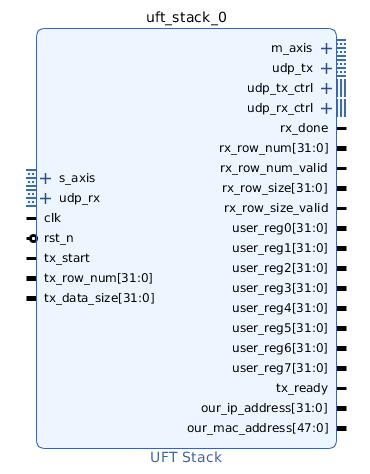
\includegraphics[width=0.5\textwidth] {images/dataflow/uftcorestream.png}
    \caption{UFT IP core with AXI4-Stream interface}
    \label{fig:uftipcoreaxistream}
\end{figure}
% ==============================================================================
%                             Control
% ==============================================================================
\section{Control} \label{ch:control}
Now that the image data is received by the UFT core it has to be sent to the
Wallis filter in the right order. Reordering the pixel data is the main task of
the controller besides caching data and controlling the UFT and wallis cores. 

As already mentioned at the beginning of chapter \ref{chapt:dataflow} two
implementations were realized. Solution A was implemented using Vivado HLS and
is documented in chapter \ref{ch:controller:hls} followed by solution B written
in VHDL and delineated in chapter \ref{ch:controller:vhdl}. The problem is
stated in the following chapter.

% ==============================================================================
%                             Concept
% ==============================================================================
\subsection{Concept} \label{ch:control:concept}
Image data comming from the PC is sent row wise with the left most pixel sent
first. This is due to the fact that OpenCV (which is used on PC side to access
images) stores the image data in said layout \cite{opencv_structures}. The
Wallis filter however, requires its input data to be coloumn wise with the top
most pixel sent first as described in chapter \ref{ch:ip:concept}. Figure 
\ref{fig:memproblem} illustrates this issue. The blue ``write'' arrow shows the data
comming from the UFT core and the red ``read'' arrow represents the order the
data has to be sent to the Wallis filter. For illustration purposes a window
length of five and image width of eight was used.

\begin{figure}[H]
    \centering
    \begin{adjustbox}{scale=0.7}
        % \tikzsetnextfilename{system-overview}
\begin{tikzpicture}[
    rounded corners=0mm,
    triangle/.style = {fill=blue!20, regular polygon, regular polygon sides=3 },
    node rotated/.style = {rotate=180},
    border rotated/.style = {shape border rotate=180}
]
    %coordinates
    \coordinate (orig)      at (0,0);

    \begin{pgfonlayer}{main}
        
        % Write arrows
        % \draw[draw=blue,line width=1.5mm] (8,4.5) .. controls (8,4) and (-1,4) .. (-1,3.5);
        % \path[draw=blue,line width=1.5mm] ($(-1,3.5)$) -- ($(8,3.5)$) node[anchor=east] {};

        % Write path
        \path[draw={rgb:red,1;green,2;blue,3},line width=1.0mm] ($(-2,4.5)$)  -- ($(9,4.5)$);
        \path[draw={rgb:red,1;green,2;blue,3},line width=1.0mm]  (-1,3.5) -- ($(9,3.5)$) ;
        \path[draw={rgb:red,1;green,2;blue,3},line width=1.0mm]  (-1,2.5) -- ($(9,2.5)$) ;
        \path[draw={rgb:red,1;green,2;blue,3},line width=1.0mm]  (-1,1.5) -- ($(9,1.5)$) ;
        \path[draw={rgb:red,1;green,2;blue,3},line width=1.0mm]  (-1,0.5) -- ($(9,0.5)$);
        \path[draw={rgb:red,1;green,2;blue,3},line width=1.0mm,dashed] ($(9,4.5)$)  .. controls (9,4) and (-1,4) .. (-1,3.5);
        \path[draw={rgb:red,1;green,2;blue,3},line width=1.0mm,dashed] ($(9,3.5)$)  .. controls (9,3) and (-1,3) .. (-1,2.5);
        \path[draw={rgb:red,1;green,2;blue,3},line width=1.0mm,dashed] ($(9,2.5)$)  .. controls (9,2) and (-1,2) .. (-1,1.5);
        \path[draw={rgb:red,1;green,2;blue,3},line width=1.0mm,dashed] ($(9,1.5)$)  .. controls (9,1) and (-1,1) .. (-1,0.5);
        % Write triangles
        \node[triangle,shape border rotate=270, fill={rgb:red,1;green,2;blue,3},minimum size=0.1cm] at (-1,0.5) {};
        \node[triangle,shape border rotate=270, fill={rgb:red,1;green,2;blue,3},minimum size=0.1cm] at (-1,1.5) {};
        \node[triangle,shape border rotate=270, fill={rgb:red,1;green,2;blue,3},minimum size=0.1cm] at (-1,2.5) {};
        \node[triangle,shape border rotate=270, fill={rgb:red,1;green,2;blue,3},minimum size=0.1cm] at (-1,3.5) {};
        \node[triangle,shape border rotate=270, fill={rgb:red,1;green,2;blue,3},minimum size=0.1cm] at (-1,4.5) {};
        
        % Read path
        \path[draw={rgb:red,3;green,1;blue,2},line width=1.0mm]  (0.5,6)  -- (0.5,-0.5);
        \path[draw={rgb:red,3;green,1;blue,2},line width=1.0mm]  (1.5,5.5)  -- (1.5,-0.5);
        \path[draw={rgb:red,3;green,1;blue,2},line width=1.0mm]  (2.5,5.5)  -- (2.5,-0.5);
        \path[draw={rgb:red,3;green,1;blue,2},line width=1.0mm]  (3.5,5.5)  -- (3.5,-0.5);
        \path[draw={rgb:red,3;green,1;blue,2},line width=1.0mm]  (4.5,5.5)  -- (4.5,-0.5);

        \path[draw={rgb:red,3;green,1;blue,2},line width=1.0mm,dashed] (0.5,-0.5)  .. controls (1,-0.5) and (1,5.5) .. (1.5,5.5);
        \path[draw={rgb:red,3;green,1;blue,2},line width=1.0mm,dashed] (1.5,-0.5)  .. controls (2,-0.5) and (2,5.5) .. (2.5,5.5);
        \path[draw={rgb:red,3;green,1;blue,2},line width=1.0mm,dashed] (2.5,-0.5)  .. controls (3,-0.5) and (3,5.5) .. (3.5,5.5);
        \path[draw={rgb:red,3;green,1;blue,2},line width=1.0mm,dashed] (3.5,-0.5)  .. controls (4,-0.5) and (4,5.5) .. (4.5,5.5);
        % Read triangles
        \node[triangle, border rotated, fill={rgb:red,3;green,1;blue,2},minimum size=0.1cm] at (0.5,5.5) {};
        \node[triangle, border rotated, fill={rgb:red,3;green,1;blue,2},minimum size=0.1cm] at (1.5,5.5) {};
        \node[triangle, border rotated, fill={rgb:red,3;green,1;blue,2},minimum size=0.1cm] at (2.5,5.5) {};
        \node[triangle, border rotated, fill={rgb:red,3;green,1;blue,2},minimum size=0.1cm] at (3.5,5.5) {};
        \node[triangle, border rotated, fill={rgb:red,3;green,1;blue,2},minimum size=0.1cm] at (4.5,5.5) {};

        % Text
        \node[] (write) at (-2,5) {Write};
        \node[] (read) at (0,6.2) {Read};

        % Braces
        \draw [line width=0.5mm,decorate,decoration={brace,amplitude=10pt},xshift=-4pt,yshift=0pt] (9.5,5) -- (9.5,0) node [black,midway,xshift=0.5cm,anchor=west] {Window length};
        \draw [line width=0.5mm,decorate,decoration={brace,amplitude=10pt},xshift=-0pt,yshift=0pt] (8,-0.5) -- (0,-0.5) node [black,midway,yshift=-0.5cm,anchor=north] {Image width};
        
        % Center pixel
        \draw[black,line width=0.5mm] (2,2) rectangle (3,3);
        % Window size
        \draw[black,line width=0.5mm] (0,0) rectangle (5,5);
        % Axis
        \foreach \x in {0,1,2,3,4}
            \node[anchor=north] at ($(-0.5,5)-(0,\x)$)  {$\x$};

    \end{pgfonlayer}

    % Foreground
    \begin{pgfonlayer}{foreground}
        
    \end{pgfonlayer} 

    % Background
    \begin{pgfonlayer}{background}
        % Grid
        \draw[step=1cm,gray,very thin] (0,0) grid (8,5);
    \end{pgfonlayer} 

\end{tikzpicture}
    \end{adjustbox}
    \caption{Memory reordering problem}
    \label{fig:memproblem}
\end{figure}

This however is only one part of the problem. Another issue arises if the
progression of the neighbourhood accross the input image is observed. We
destinguish two scenarios: A) moving the neighbourhood horizontally to the right
and B) advancing the neighbourhood to the next row vertically. The first
scenario is illustrated in figure \ref{fig:memproblemgrowthx}. The green arrow
marks the new coloumn of the neighbourhood to be sent to the Wallis filter.

\begin{figure}[H]
    \centering
    \begin{adjustbox}{scale=0.7}
        % \tikzsetnextfilename{system-overview}
\begin{tikzpicture}[
    rounded corners=0mm,
    triangle/.style = {fill=blue!20, regular polygon, regular polygon sides=3 },
    node rotated/.style = {rotate=180},
    border rotated/.style = {shape border rotate=180}
]
    %coordinates
    \coordinate (orig)      at (0,0);

    \begin{pgfonlayer}{main}
        
        % Write arrows
        % \draw[draw=blue,line width=1.5mm] (8,4.5) .. controls (8,4) and (-1,4) .. (-1,3.5);
        % \path[draw=blue,line width=1.5mm] ($(-1,3.5)$) -- ($(8,3.5)$) node[anchor=east] {};

        % Write path
        % \path[draw={rgb:red,1;green,2;blue,3},line width=1.0mm] ($(-2,4.5)$)  -- ($(9,4.5)$);
        % \path[draw={rgb:red,1;green,2;blue,3},line width=1.0mm]  (-1,3.5) -- ($(9,3.5)$) ;
        % \path[draw={rgb:red,1;green,2;blue,3},line width=1.0mm]  (-1,2.5) -- ($(9,2.5)$) ;
        % \path[draw={rgb:red,1;green,2;blue,3},line width=1.0mm]  (-1,1.5) -- ($(9,1.5)$) ;
        % \path[draw={rgb:red,1;green,2;blue,3},line width=1.0mm]  (-1,0.5) -- ($(9,0.5)$);
        % \path[draw={rgb:red,1;green,2;blue,3},line width=1.0mm,dashed] ($(9,4.5)$)  .. controls (9,4) and (-1,4) .. (-1,3.5);
        % \path[draw={rgb:red,1;green,2;blue,3},line width=1.0mm,dashed] ($(9,3.5)$)  .. controls (9,3) and (-1,3) .. (-1,2.5);
        % \path[draw={rgb:red,1;green,2;blue,3},line width=1.0mm,dashed] ($(9,2.5)$)  .. controls (9,2) and (-1,2) .. (-1,1.5);
        % \path[draw={rgb:red,1;green,2;blue,3},line width=1.0mm,dashed] ($(9,1.5)$)  .. controls (9,1) and (-1,1) .. (-1,0.5);
        % % Write triangles
        % \node[triangle,shape border rotate=270, fill={rgb:red,1;green,2;blue,3},minimum size=0.1cm] at (-1,0.5) {};
        % \node[triangle,shape border rotate=270, fill={rgb:red,1;green,2;blue,3},minimum size=0.1cm] at (-1,1.5) {};
        % \node[triangle,shape border rotate=270, fill={rgb:red,1;green,2;blue,3},minimum size=0.1cm] at (-1,2.5) {};
        % \node[triangle,shape border rotate=270, fill={rgb:red,1;green,2;blue,3},minimum size=0.1cm] at (-1,3.5) {};
        % \node[triangle,shape border rotate=270, fill={rgb:red,1;green,2;blue,3},minimum size=0.1cm] at (-1,4.5) {};
        
        % Read path
        \path[draw={rgb:red,3;green,1;blue,2},line width=1.0mm]  (0.5,6)  -- (0.5,-0.5);
        \path[draw={rgb:red,3;green,1;blue,2},line width=1.0mm]  (1.5,5.5)  -- (1.5,-0.5);
        \path[draw={rgb:red,3;green,1;blue,2},line width=1.0mm]  (2.5,5.5)  -- (2.5,-0.5);
        \path[draw={rgb:red,3;green,1;blue,2},line width=1.0mm]  (3.5,5.5)  -- (3.5,-0.5);
        \path[draw={rgb:red,3;green,1;blue,2},line width=1.0mm]  (4.5,5.5)  -- (4.5,-0.5);

        \path[draw={rgb:red,3;green,1;blue,2},line width=1.0mm,dashed] (0.5,-0.5)  .. controls (1,-0.5) and (1,5.5) .. (1.5,5.5);
        \path[draw={rgb:red,3;green,1;blue,2},line width=1.0mm,dashed] (1.5,-0.5)  .. controls (2,-0.5) and (2,5.5) .. (2.5,5.5);
        \path[draw={rgb:red,3;green,1;blue,2},line width=1.0mm,dashed] (2.5,-0.5)  .. controls (3,-0.5) and (3,5.5) .. (3.5,5.5);
        \path[draw={rgb:red,3;green,1;blue,2},line width=1.0mm,dashed] (3.5,-0.5)  .. controls (4,-0.5) and (4,5.5) .. (4.5,5.5);
        % Read triangles
        \node[triangle, border rotated, fill={rgb:red,3;green,1;blue,2},minimum size=0.1cm] at (0.5,5.5) {};
        \node[triangle, border rotated, fill={rgb:red,3;green,1;blue,2},minimum size=0.1cm] at (1.5,5.5) {};
        \node[triangle, border rotated, fill={rgb:red,3;green,1;blue,2},minimum size=0.1cm] at (2.5,5.5) {};
        \node[triangle, border rotated, fill={rgb:red,3;green,1;blue,2},minimum size=0.1cm] at (3.5,5.5) {};
        \node[triangle, border rotated, fill={rgb:red,3;green,1;blue,2},minimum size=0.1cm] at (4.5,5.5) {};

        % Text
        % \node[] (write) at (-2,5) {Write};
        \node[] (read) at (0,6.2) {Read};

        % Braces
        \draw [line width=0.5mm,decorate,decoration={brace,amplitude=10pt},xshift=-4pt,yshift=0pt] (9.5,5) -- (9.5,0) node [black,midway,xshift=0.5cm,anchor=west] {Window size};
        \draw [line width=0.5mm,decorate,decoration={brace,amplitude=10pt},xshift=-0pt,yshift=0pt] (8,-0.5) -- (0,-0.5) node [black,midway,yshift=-0.5cm,anchor=north] {Image width};
        
        % Center pixel
        \draw[black,line width=0.5mm] (3,2) rectangle (4,3);
        % Window size
        \draw[black,line width=0.5mm] (1,0) rectangle (6,5);

        % Growth X
        \path[draw={rgb:red,1;green,3;blue,1},line width=1.0mm]  (5.5,5.5)  -- (5.5,-0.5);
        \path[draw={rgb:red,1;green,3;blue,1},line width=1.0mm,dashed] (4.5,-0.5)  .. controls (5,-0.5) and (5,5.5) .. (5.5,5.5);
        \node[triangle, border rotated, fill={rgb:red,1;green,3;blue,1},minimum size=0.1cm] at (5.5,5.5) {};

        % Axis
        \foreach \x in {0,1,2,3,4}
            \node[anchor=north] at ($(-0.5,5)-(0,\x)$)  {$\x$};
    \end{pgfonlayer}

    % Foreground
    \begin{pgfonlayer}{foreground}
        
    \end{pgfonlayer} 

    % Background
    \begin{pgfonlayer}{background}
        % Grid
        \draw[step=1cm,gray,very thin] (0,0) grid (8,5);
    \end{pgfonlayer} 

\end{tikzpicture}
    \end{adjustbox}
    \caption{Scenario A) Data growth in horizontal direction}
    \label{fig:memproblemgrowthx}
\end{figure}

This progression is made for each coloumn of the input image until the last
coloumn was processed. Then scenario B) comes to play. Moving the neighbourhood
vertically to the next row by one pixel requires new image data of one row
and $WINDOW\_LENGTH-1$ rows of image data that had already been processed on the
previous row. Figure \ref{fig:memproblemgrowthy} illustrates scenario B.

\begin{figure}[H]
    \centering
    \begin{adjustbox}{scale=0.7}
        % \tikzsetnextfilename{system-overview}
\begin{tikzpicture}[
    rounded corners=0mm,
    triangle/.style = {fill=blue!20, regular polygon, regular polygon sides=3 },
    node rotated/.style = {rotate=180},
    border rotated/.style = {shape border rotate=180}
]
    %coordinates
    \coordinate (orig)      at (0,0);

    \begin{pgfonlayer}{main}
        
        % Write arrows
        % \draw[draw=blue,line width=1.5mm] (8,4.5) .. controls (8,4) and (-1,4) .. (-1,3.5);
        % \path[draw=blue,line width=1.5mm] ($(-1,3.5)$) -- ($(8,3.5)$) node[anchor=east] {};

        % Write path
        \path[draw={rgb:red,1;green,3;blue,1},line width=1.0mm] ($(-2,0.5)$)  -- ($(9,0.5)$);
        % Write triangles
        \node[triangle,shape border rotate=270, fill={rgb:red,1;green,3;blue,1},minimum size=0.1cm] at (-1,0.5) {};
        
        % Read path
        \path[draw={rgb:red,3;green,1;blue,2},line width=1.0mm]  (0.5,6)  -- (0.5,-0.5);
        \path[draw={rgb:red,3;green,1;blue,2},line width=1.0mm]  (1.5,5.5)  -- (1.5,-0.5);
        \path[draw={rgb:red,3;green,1;blue,2},line width=1.0mm]  (2.5,5.5)  -- (2.5,-0.5);
        \path[draw={rgb:red,3;green,1;blue,2},line width=1.0mm]  (3.5,5.5)  -- (3.5,-0.5);
        \path[draw={rgb:red,3;green,1;blue,2},line width=1.0mm]  (4.5,5.5)  -- (4.5,-0.5);

        \path[draw={rgb:red,3;green,1;blue,2},line width=1.0mm,dashed] (0.5,-0.5)  .. controls (1,-0.5) and (1,5.5) .. (1.5,5.5);
        \path[draw={rgb:red,3;green,1;blue,2},line width=1.0mm,dashed] (1.5,-0.5)  .. controls (2,-0.5) and (2,5.5) .. (2.5,5.5);
        \path[draw={rgb:red,3;green,1;blue,2},line width=1.0mm,dashed] (2.5,-0.5)  .. controls (3,-0.5) and (3,5.5) .. (3.5,5.5);
        \path[draw={rgb:red,3;green,1;blue,2},line width=1.0mm,dashed] (3.5,-0.5)  .. controls (4,-0.5) and (4,5.5) .. (4.5,5.5);
        % Read triangles
        \node[triangle, border rotated, fill={rgb:red,3;green,1;blue,2},minimum size=0.1cm] at (0.5,5.5) {};
        \node[triangle, border rotated, fill={rgb:red,3;green,1;blue,2},minimum size=0.1cm] at (1.5,5.5) {};
        \node[triangle, border rotated, fill={rgb:red,3;green,1;blue,2},minimum size=0.1cm] at (2.5,5.5) {};
        \node[triangle, border rotated, fill={rgb:red,3;green,1;blue,2},minimum size=0.1cm] at (3.5,5.5) {};
        \node[triangle, border rotated, fill={rgb:red,3;green,1;blue,2},minimum size=0.1cm] at (4.5,5.5) {};

        % Text
        \node[] (write) at (-2,1) {Write};
        \node[] (read) at (0,6.2) {Read};

        % Braces
        \draw [line width=0.5mm,decorate,decoration={brace,amplitude=10pt},xshift=-4pt,yshift=0pt] (9.5,5) -- (9.5,0) node [black,midway,xshift=0.5cm,anchor=west] {Window size};
        \draw [line width=0.5mm,decorate,decoration={brace,amplitude=10pt},xshift=-0pt,yshift=0pt] (8,-0.5) -- (0,-0.5) node [black,midway,yshift=-0.5cm,anchor=north] {Image width};
        
        % Center pixel
        \draw[black,line width=0.5mm] (2,2) rectangle (3,3);
        % Window size
        \draw[black,line width=0.5mm] (0,0) rectangle (5,5);

        % Axis
        \foreach \x in {0,1,2,3,4,5}
            \node[anchor=north] at ($(-0.5,6)-(0,\x)$)  {$\x$};
    \end{pgfonlayer}

    % Foreground
    \begin{pgfonlayer}{foreground}
        
    \end{pgfonlayer} 

    % Background
    \begin{pgfonlayer}{background}
        % Grid
        \draw[step=1cm,gray,very thin] (0,0) grid (8,6);
    \end{pgfonlayer} 

\end{tikzpicture}
    \end{adjustbox}
    \caption{Scenario B) Data growth in vertical direction}
    \label{fig:memproblemgrowthy}
\end{figure}

From these two scenarios we can conclude two problems the controller has to
solve:
\begin{itemize}
    \item Send the image data in the right order (coloumn wise with
    $WINDOW\_LENGTH$ sized coloumns)
    \item Cache $WINDOW\_LENGTH-1$ rows for the computation of the next image
    row
\end{itemize}

In addition the controller has to start the UFT transmission if an image row has
been processed and configure the Wallis filter with the appropriate parameters.

\clearpage

% ==============================================================================
%                             HLS
% ==============================================================================
\subsection{Implementation HLS} \label{ch:controller:hls}
Now that the problems are analysed, the proceeding can be stated. For the first
solution a approach using Vivado HLS was picked. The main motivations for this
decision were the fact that we learned how fast we can have a working IP core
using the Vivado HLS workflow and that we wanted to test the ability to
implement a state machine in Vivado HLS. In the following chapters the
requirements for this state machine are listed, a brief insight into the source
code is given and the main hurdles while developing the core are unfold.

\subsubsection*{Requirements}
Besides the dataflow described in \ref{ch:control:concept} the IP core
interfaces must be defined. Table \ref{tab:controlleraports} lists the IP
interfaces as defined in \texttt{controller.cpp}.

\begin{table}[b!]
    \centering
    \begin{tabular}{l l l p{8cm}}
        \toprule
        Variable & Type & Connection to & Description \\
        \midrule
        \texttt{memp} & \texttt{AXI4 Master} & Memory &
        Access to the block memory where the image data is stored
        \\
        \texttt{cbus} & \texttt{AXI4 Master} & UFT core &
        Control the AXI4-Lite slave registers to control the UFT core
        \\
        \texttt{inData} & \texttt{AXI4-Stream} & Wallis filter &
        Processed pixels comming from the Wallis filter
        \\
        \texttt{outData} & \texttt{AXI4-Stream} & Wallis filter &
        Image data sent to the Wallis filter for processing
        \\
        \texttt{rx\_done} & \texttt{ap\_uint<1>} & UFT core &
        Is asserted after a file transfer is complete
        \\
        \texttt{tx\_ready} & \texttt{ap\_uint<1>} & UFT core &
        Is asserted if UFT core is ready to send
        \\
        \bottomrule
    \end{tabular}
    \caption{Controller solution A interface ports}
    \label{tab:controlleraports}
\end{table}

The IP core implements a finite state machine as seen in figure 
\ref{fig:controllerfsm}. After the initial state
\texttt{S\_INIT} where the UFT core is initialized the state machine goes to its
idle state \texttt{S\_IDLE}. If the UFT core indicates the end of a file
transfer the image width is stored and the state machine switches to the 
\texttt{S\_READ} state. There it fills the first junk of its buffers and
switches to the \texttt{S\_STREAM} state. Now the data is sent from the
internal buffers to the Wallis filter in the correct order. Simultaneously the
processed pixels from the Wallis filter are stored inside a memory. If all
pixels in one line are processed the state \texttt{S\_WRITE} is activated. The
processed pixels are stored in block memory using the \texttt{memp} AXI4 Master
interface and the state machine switches to the \texttt{S\_WAIT\_TO\_SEND}
state. If the UFT core Tx is ready, the state \texttt{S\_SEND} is activated
where the UFT core is configured and a transmission is started.

\begin{figure}[H]
    \centering
    \begin{adjustbox}{scale=1}
        % \tikzsetnextfilename{system-overview}
\begin{tikzpicture}[->,>=stealth',shorten >=1pt,auto,node distance=2.8cm,
                    semithick]

    \tikzstyle{every state}=[fill=white,draw=black,text=black,minimum width=1cm]
    
    % states
    \node[initial,state] (A)                    {INIT};
    \node[state]         (B) [right of=A]       {IDLE};
    \node[state]         (C) [above right of=B] {READ};
    \node[state]         (D) [right of=C]       {STREAM};
    \node[state]         (E) [below right of=D]       {WRITE};
    \node[state, align=center]         (F) [below left of=E]       {WAIT\_TO\_ \\ SEND};
    \node[state]         (G) [left of=F]       {SEND};


    % path
    \path   (A) edge              node {} (B)
            (B) edge              node {} (C)
            (C) edge              node {} (D)
            (D) edge              node {} (E)
            (E) edge              node {} (F)
            (F) edge              node {} (G)
            (G) edge              node {} (B);
    \begin{pgfonlayer}{main}

    \end{pgfonlayer}

    \begin{pgfonlayer}{foreground}
    
    \end{pgfonlayer} 


\end{tikzpicture}
    \end{adjustbox}
    \caption{Controller solution A simplified state machine}
    \label{fig:controllerfsm}
\end{figure}

\subsubsection*{Realization}
\todo[inline]{Graphic for memory layout solution A}
According to Xilinx application note XAPP-1209 \cite{xapp1209} a state
machine in Vivado HLS can be realizes by using a switch statement in the C code.
The code in file \texttt{controller.cpp} implements the state machine behaviour.
The state machine code is very straight foreward. More work went into the memory
layout. Because the memory bus to read and write pixels to and from memory is
AXI4 based, single byte access result in considerably less throughput than
burst access.
To take advantage of these burst accesses, a ping-pong buffer structure was
realized. There are two buffers, each of the size of $WINDOW\_LENGTH *
AXI\_BURST\_SIZE$ bytes, where $AXI\_BURST\_SIZE$ represents the number of bytes
read
in one burst access. It requires $WINDOW\_LENGTH$ burst reads to fill one
buffer. If one buffer is filled, it can be accessed by single byte access to
read the data in the required order for the Wallis filter, as shown in figure
\ref{fig:memproblem}. During the time the data is read from one buffer, the
other buffer is filled with image data from the AXI4 bus, hence the name
ping-pong buffer. Filling the buffer is done in the \texttt{fillBuff} routine
as shown on listing \ref{lst:buf_fill}:

\begin{minipage}{\textwidth}
\begin{lstlisting}[style=CStyle, caption=Buffer fill simplified,
label=lst:buf_fill]
void fillBuff(volatile uint8_t *memp, volatile uint8_t *buf,
    uint32_t imgWidth, uint32_t off)
{
    uint32_t i, inOff, outOff;
    for(i = 0; i < WINDOW_LEN; i++)
    {
        inOff = off + i*imgWidth;
        outOff = i*AXI_BURST_SIZE;
        memcpy(&buf[outOff], &memp[inOff], AXI_BURST_SIZE);
    }
}\end{lstlisting}
\end{minipage}


\subsubsection*{Hurdles}

\subsubsection*{Conclusion}
\todo[inline]{ILA measurement showing slow output pixels}

\subsubsection*{IF-Statement} \label{ch:data:if}

% \begin{minipage}{\textwidth}
% \begin{lstlisting}[style=CStyle, caption=Buffer switching reloading without else statement, label=lst:buf_false]
% if( (outPpBuf == ppBufA) && (ms_pctr < (inLineSize-PIN_PONG_BUF_SIZE)) ) {
%     if(!ppBufBrdy) {
%         ...
%     }
% }
% if( (outPpBuf == ppBufB) && (ms_pctr < (inLineSize-PIN_PONG_BUF_SIZE)) ) {
%     if(!ppBufArdy) {
%         ...
%     }
% }
% \end{lstlisting}
% \end{minipage}

% \begin{minipage}{\textwidth}
% \begin{lstlisting}[style=CStyle, caption=Buffer switching reloading with else statement, label=lst:buf_right]
% if (ms_pctr < (inLineSize-PIN_PONG_BUF_SIZE)) {
% 	if( (outPpBuf == ppBufA)  ) {
% 		if(!ppBufBrdy) {
% 			...
% 		}
% 	}
% 	else {
% 		if(!ppBufArdy) {
% 			...
% 		}
% 	}
% }
% \end{lstlisting}
% \end{minipage}

% ==============================================================================
%                             VHDL
% ==============================================================================
\subsection{Implementation VHDL} \label{ch:controller:vhdl}
